\documentclass[dvipdfmx]{beamer}
\usetheme{metropolis}           % Use metropolis theme
\usepackage{float}
\usepackage{tikz}
\usepackage{amsmath,amssymb,bm}
\usetikzlibrary {arrows.meta}
\usetikzlibrary {bending}
\usepackage{listings,jvlisting} %日本語のコメントアウトをする場合jvlisting(もしくはjlisting)が必要
%ここからソースコードの表示に関する設定
\lstset{
  basicstyle={\ttfamily},
  identifierstyle={\small},
  commentstyle={\smallitshape},
  keywordstyle={\small\bfseries},
  ndkeywordstyle={\small},
  stringstyle={\small\ttfamily},
  frame={tb},
  breaklines=true,
  columns=[l]{fullflexible},
  numbers=left,
  xrightmargin=0zw,
  xleftmargin=3zw,
  numberstyle={\scriptsize},
  stepnumber=1,
  numbersep=1zw,
  lineskip=-0.5ex
}

\title{Progress}
\date{\today}
\author{Mizuno Yasuaki}
%\institute{Centre for Modern Beamer Themes}
\begin{document}
  \maketitle
  
  \begin{frame}{目次}
    \begin{enumerate}
      \item 研究内容
      \item アミノ酸配列の画像の作成
      \item アミノ酸配列の画像を用いた機械学習
      \item 学習結果
    \end{enumerate} 
  \end{frame}

  \begin{frame}{研究内容}
    『アミノ酸配列の画像を用いた機械学習によるタンパク質ファミリー
    \footnote{
      \begin{itemize}
        \item 進化的類縁関係を持つタンパク質のグループ
        \item 共通の機能を持つタンパク質のグループ
      \end{itemize}
    }
    分類』\\
    $\rightarrow$ アミノ酸配列の画像からタンパク質ファミリーを予測する
  \end{frame}

  \begin{frame}{アミノ酸配列の画像の作成①}
    二十種のアミノ酸それぞれに単位ベクトルを図\ref{fig:amino_vector}のように割り当てる。
    右のアミノ酸ほど親水性度が大きい。
    \begin{figure}
      \centering
      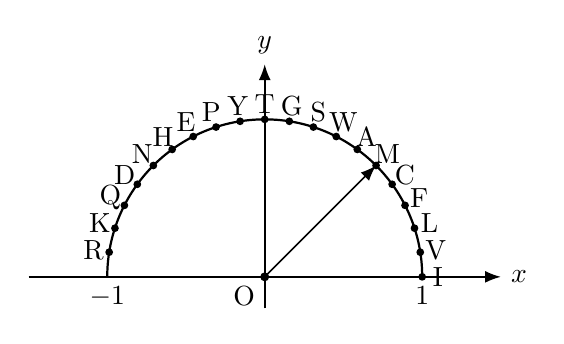
\begin{tikzpicture}[scale=2]
        \coordinate (O) at (0, 0);
        \coordinate (A) at (1, 0);
        \coordinate (B) at (-1, 0);

        \draw [arrows = {-Latex[scale=1]}, semithick] (-1.5, 0)--(1.5, 0) node [right] {$x$};
        \draw [arrows = {-Latex[scale=1]}, semithick] (0, -0.2)--(0, 1.35) node [above] {$y$};
        
        \foreach \t / \aminolabel in {0/I, 1/V, 2/L, 3/F, 4/C, 5/M, 6/A, 7/W, 8/S, 9/G, 10/T, 11/Y, 12/P, 13/E, 14/H, 15/N, 16/D, 17/Q, 18/K, 19/R}{
          \draw ({1.1 * cos(9 * \t)}, {1.1 * sin(9 * \t)}) node {\aminolabel};
          \fill ({cos(9 * \t)}, {sin(9 * \t)}) circle [radius=0.7pt];
        }

        \filldraw (0, 0) circle [radius=0.7pt] node [below left] {$\mathrm{O}$};
        \draw (A) node [below] {$1$};
        \draw (B) node [below] {$-1$};
        \draw [thick] (A) arc (0:180:1);
        \draw [arrows = {-Latex[scale=1]}, semithick] (O)--({cos(9 * 5)}, {sin(9 * 5)});
      \end{tikzpicture}
      \caption{amino vector}
      \label{fig:amino_vector}
    \end{figure}
  \end{frame}

  \begin{frame}{アミノ酸配列の画像の作成②}
    アミノ酸配列で出現したアミノ酸に対応するベクトルを足していき、グラフを作成する。\\
    ex)アミノ酸配列:MTI
    \begin{figure}
      \centering
      \includegraphics[keepaspectratio, scale=0.5]{images/example.png}
      \caption{example}
    \end{figure}
  \end{frame}

  \begin{frame}{アミノ酸配列の画像を用いた機械学習}
    \href{https://www.nri.com/jp/knowledge/glossary/lst/ka/machine_learning}{機械学習}とは、データを分析する方法の一つで、データから自動で学習し、
    データの背景にあるパターンを発見する方法。学習した成果に基づいて
    「予測・判断」する。研究ではアミノ酸配列の画像とそれに対応するファミリーを学習し、アミノ酸配列の画像のファミリーを予測する。
  \end{frame}

  \begin{frame}{学習結果}
    最も単純な全結合ニューラルネットワークを使用。
  \end{frame}

  \begin{frame}{今後の予定}
    \begin{itemize}
      \item より精度を高めるために試行錯誤する
      \begin{itemize}
        \item 画像の作成方法を見直す
        \item 様々なニューラルネットワークを試す
      \end{itemize}
    \end{itemize}
  \end{frame}
\end{document}


